% Options for packages loaded elsewhere
\PassOptionsToPackage{unicode}{hyperref}
\PassOptionsToPackage{hyphens}{url}
\documentclass[
]{article}
\usepackage{xcolor}
\usepackage[margin=1in]{geometry}
\usepackage{amsmath,amssymb}
\setcounter{secnumdepth}{-\maxdimen} % remove section numbering
\usepackage{iftex}
\ifPDFTeX
  \usepackage[T1]{fontenc}
  \usepackage[utf8]{inputenc}
  \usepackage{textcomp} % provide euro and other symbols
\else % if luatex or xetex
  \usepackage{unicode-math} % this also loads fontspec
  \defaultfontfeatures{Scale=MatchLowercase}
  \defaultfontfeatures[\rmfamily]{Ligatures=TeX,Scale=1}
\fi
\usepackage{lmodern}
\ifPDFTeX\else
  % xetex/luatex font selection
\fi
% Use upquote if available, for straight quotes in verbatim environments
\IfFileExists{upquote.sty}{\usepackage{upquote}}{}
\IfFileExists{microtype.sty}{% use microtype if available
  \usepackage[]{microtype}
  \UseMicrotypeSet[protrusion]{basicmath} % disable protrusion for tt fonts
}{}
\makeatletter
\@ifundefined{KOMAClassName}{% if non-KOMA class
  \IfFileExists{parskip.sty}{%
    \usepackage{parskip}
  }{% else
    \setlength{\parindent}{0pt}
    \setlength{\parskip}{6pt plus 2pt minus 1pt}}
}{% if KOMA class
  \KOMAoptions{parskip=half}}
\makeatother
\usepackage{color}
\usepackage{fancyvrb}
\newcommand{\VerbBar}{|}
\newcommand{\VERB}{\Verb[commandchars=\\\{\}]}
\DefineVerbatimEnvironment{Highlighting}{Verbatim}{commandchars=\\\{\}}
% Add ',fontsize=\small' for more characters per line
\usepackage{framed}
\definecolor{shadecolor}{RGB}{248,248,248}
\newenvironment{Shaded}{\begin{snugshade}}{\end{snugshade}}
\newcommand{\AlertTok}[1]{\textcolor[rgb]{0.94,0.16,0.16}{#1}}
\newcommand{\AnnotationTok}[1]{\textcolor[rgb]{0.56,0.35,0.01}{\textbf{\textit{#1}}}}
\newcommand{\AttributeTok}[1]{\textcolor[rgb]{0.13,0.29,0.53}{#1}}
\newcommand{\BaseNTok}[1]{\textcolor[rgb]{0.00,0.00,0.81}{#1}}
\newcommand{\BuiltInTok}[1]{#1}
\newcommand{\CharTok}[1]{\textcolor[rgb]{0.31,0.60,0.02}{#1}}
\newcommand{\CommentTok}[1]{\textcolor[rgb]{0.56,0.35,0.01}{\textit{#1}}}
\newcommand{\CommentVarTok}[1]{\textcolor[rgb]{0.56,0.35,0.01}{\textbf{\textit{#1}}}}
\newcommand{\ConstantTok}[1]{\textcolor[rgb]{0.56,0.35,0.01}{#1}}
\newcommand{\ControlFlowTok}[1]{\textcolor[rgb]{0.13,0.29,0.53}{\textbf{#1}}}
\newcommand{\DataTypeTok}[1]{\textcolor[rgb]{0.13,0.29,0.53}{#1}}
\newcommand{\DecValTok}[1]{\textcolor[rgb]{0.00,0.00,0.81}{#1}}
\newcommand{\DocumentationTok}[1]{\textcolor[rgb]{0.56,0.35,0.01}{\textbf{\textit{#1}}}}
\newcommand{\ErrorTok}[1]{\textcolor[rgb]{0.64,0.00,0.00}{\textbf{#1}}}
\newcommand{\ExtensionTok}[1]{#1}
\newcommand{\FloatTok}[1]{\textcolor[rgb]{0.00,0.00,0.81}{#1}}
\newcommand{\FunctionTok}[1]{\textcolor[rgb]{0.13,0.29,0.53}{\textbf{#1}}}
\newcommand{\ImportTok}[1]{#1}
\newcommand{\InformationTok}[1]{\textcolor[rgb]{0.56,0.35,0.01}{\textbf{\textit{#1}}}}
\newcommand{\KeywordTok}[1]{\textcolor[rgb]{0.13,0.29,0.53}{\textbf{#1}}}
\newcommand{\NormalTok}[1]{#1}
\newcommand{\OperatorTok}[1]{\textcolor[rgb]{0.81,0.36,0.00}{\textbf{#1}}}
\newcommand{\OtherTok}[1]{\textcolor[rgb]{0.56,0.35,0.01}{#1}}
\newcommand{\PreprocessorTok}[1]{\textcolor[rgb]{0.56,0.35,0.01}{\textit{#1}}}
\newcommand{\RegionMarkerTok}[1]{#1}
\newcommand{\SpecialCharTok}[1]{\textcolor[rgb]{0.81,0.36,0.00}{\textbf{#1}}}
\newcommand{\SpecialStringTok}[1]{\textcolor[rgb]{0.31,0.60,0.02}{#1}}
\newcommand{\StringTok}[1]{\textcolor[rgb]{0.31,0.60,0.02}{#1}}
\newcommand{\VariableTok}[1]{\textcolor[rgb]{0.00,0.00,0.00}{#1}}
\newcommand{\VerbatimStringTok}[1]{\textcolor[rgb]{0.31,0.60,0.02}{#1}}
\newcommand{\WarningTok}[1]{\textcolor[rgb]{0.56,0.35,0.01}{\textbf{\textit{#1}}}}
\usepackage{longtable,booktabs,array}
\newcounter{none} % for unnumbered tables
\usepackage{calc} % for calculating minipage widths
% Correct order of tables after \paragraph or \subparagraph
\usepackage{etoolbox}
\makeatletter
\patchcmd\longtable{\par}{\if@noskipsec\mbox{}\fi\par}{}{}
\makeatother
% Allow footnotes in longtable head/foot
\IfFileExists{footnotehyper.sty}{\usepackage{footnotehyper}}{\usepackage{footnote}}
\makesavenoteenv{longtable}
\usepackage{graphicx}
\makeatletter
\newsavebox\pandoc@box
\newcommand*\pandocbounded[1]{% scales image to fit in text height/width
  \sbox\pandoc@box{#1}%
  \Gscale@div\@tempa{\textheight}{\dimexpr\ht\pandoc@box+\dp\pandoc@box\relax}%
  \Gscale@div\@tempb{\linewidth}{\wd\pandoc@box}%
  \ifdim\@tempb\p@<\@tempa\p@\let\@tempa\@tempb\fi% select the smaller of both
  \ifdim\@tempa\p@<\p@\scalebox{\@tempa}{\usebox\pandoc@box}%
  \else\usebox{\pandoc@box}%
  \fi%
}
% Set default figure placement to htbp
\def\fps@figure{htbp}
\makeatother
\ifLuaTeX
  \usepackage{luacolor}
  \usepackage[soul]{lua-ul}
\else
  \usepackage{soul}
\fi
\setlength{\emergencystretch}{3em} % prevent overfull lines
\providecommand{\tightlist}{%
  \setlength{\itemsep}{0pt}\setlength{\parskip}{0pt}}
\usepackage{bookmark}
\IfFileExists{xurl.sty}{\usepackage{xurl}}{} % add URL line breaks if available
\urlstyle{same}
% fallback for those not using the hyperref driver hyperxmp:
\makeatletter
\@ifundefined{xmpquote}{\newcommand{\xmpquote}[1]{#1}}{}
\makeatother
\hypersetup{
  pdftitle={Lab Assignment 1 - Data in R},
  pdfauthor={Carl Gladish},
  hidelinks,
  pdfcreator={LaTeX via pandoc}}

\title{Lab Assignment 1 - Data in R}
\author{Carl Gladish}
\date{Sept 2, 2026}

\begin{document}
\maketitle

\subsubsection{What Is This?}\label{what-is-this}

This lab assignment contains some instructional material along with
several tasks for you to complete using RStudio. At the end, you will
find some ``Pencil Problems'' for you to practice solving problems by
hand without R.

You should complete this lab to help prepare for upcoming quizzes and
exams in this course. The lab assignment itself will \emph{not} be
collected for grading.

\subsubsection{Lab Objectives}\label{lab-objectives}

The objectives of this lab assignment are for you to learn how:

\begin{itemize}
\tightlist
\item
  to write, preview, and knit an R notebook
\item
  install and load an R library
\item
  to explore a data frame in R
\item
  to calculate sample statistics in R
\item
  to calculate sample statistics ``by hand'' (using a calculator) and to
  understand their meaning
\end{itemize}

\subsection{1. What is an R Notebook?}\label{what-is-an-r-notebook}

This document is an example of an \emph{R notebook}. An R notebook is a
mixture of written text and R code stored in a single file (extension
.Rmd). It is written using a simple ``markdown language''. (For
instance, you can create bold text like this: \textbf{stats is fun}.)

R Notebooks are a good way to organize your work, since it makes it easy
to present your findings and to make sure your work is
\emph{reproducible} (since you can just re-run the entire notebook).

The words you are reading right now are part of a text \emph{chunk}. An
example of an R code chunk is below. To run the code, find the ``Run
Current Chunk'' button

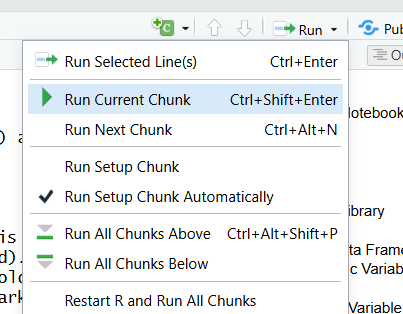
\includegraphics[width=2.36458in,height=\textheight,keepaspectratio]{images/clipboard-964275546.png}

or put the cursor anywhere inside the code chunk and use the
CTL-SHIFT-ENTER shortcut.

\begin{Shaded}
\begin{Highlighting}[]
\NormalTok{x }\OtherTok{\textless{}{-}} \DecValTok{10}
\NormalTok{y }\OtherTok{\textless{}{-}} \DecValTok{5}
\NormalTok{x}\SpecialCharTok{+}\NormalTok{y}
\end{Highlighting}
\end{Shaded}

\begin{verbatim}
## [1] 15
\end{verbatim}

At any time, you can create a \emph{preview} of an R notebook, which is
a nice-looking HTML rendering of all the text and code (and output) in
the notebook. It is a good idea to enable the \emph{Preview in Viewer
Pane} option before you click the \emph{Preview} button.

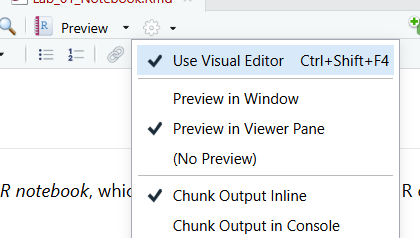
\includegraphics[width=3.125in,height=\textheight,keepaspectratio]{images/clipboard-2423193945.png}

\paragraph{Task 1}\label{task-1}

Insert an R code chunk below this text. In the code chunk, assign the
number 16 to a variable \(t\) and then evaluate \(t^2\).

\begin{Shaded}
\begin{Highlighting}[]
\NormalTok{t }\OtherTok{=} \DecValTok{16}
\NormalTok{t}\SpecialCharTok{\^{}}\DecValTok{2}
\end{Highlighting}
\end{Shaded}

\begin{verbatim}
## [1] 256
\end{verbatim}

\paragraph{Task 2}\label{task-2}

Create a preview of this notebook as it is. You should see the output in
the \emph{Viewer} pane (lower right pane of R Studio).

\begin{Shaded}
\begin{Highlighting}[]
\DecValTok{2}\SpecialCharTok{+}\DecValTok{2}
\end{Highlighting}
\end{Shaded}

\begin{verbatim}
## [1] 4
\end{verbatim}

Now run the code chunk above (with \texttt{2+2}) and then rerun Preview.
You should see the new output appear in the preview. Previewing by
itself does not force any code chunks to run.

\paragraph{Task 3}\label{task-3}

Let's say you are done creating this notebook. To create a presentable
version of the notebook, you can \emph{knit} it into several final
formats, including: HTML, pdf, and Microsoft Word.

Your task is to knit the notebook into a Microsoft Word document using
the drop-down menu next to ``Preview'' (or set the output format to WORD
and use the CTL-SHIFT-k shortcut).

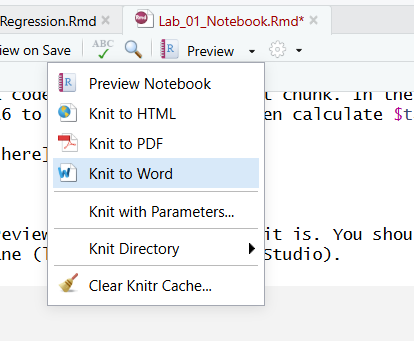
\includegraphics[width=3.03125in,height=\textheight,keepaspectratio]{images/clipboard-3953332825.png}

You will see a new Word document with your notebook content. Note that
\textbf{all} code chunks are automatically re-run before final rendering
when you knit an R notebook.

After you knit the notebook, the output type in the notebook headers
will have changed to ``word\_document'' (as shown) and you will not see
the Preview button anymore.

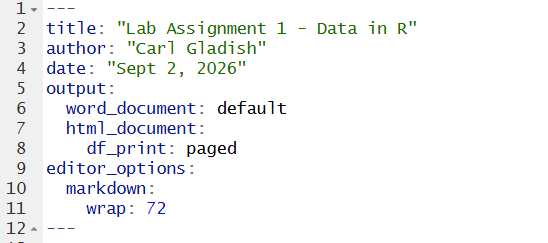
\includegraphics[width=3.86458in,height=\textheight,keepaspectratio]{images/clipboard-3758380946.png}

To enable the Preview again, manually change the output type back (as
shown):

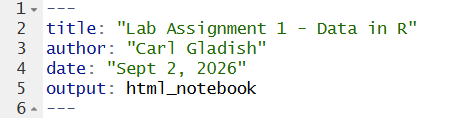
\includegraphics[width=3.85417in,height=\textheight,keepaspectratio]{images/clipboard-1066683268.png}

\paragraph{Task 4}\label{task-4}

There are two ways to type mathematical expressions in an R notebook
text chunk. The first way--let's call it the \emph{ugly} way--is just to
type it out in regular text. For instance, here is a complicated
expression written the ugly way.

sqrt(e\^{}-t - 17/2* sin( 2/3 * pi * t) )

The second way--the \emph{pretty} way--uses a separate markup language
called ``Latex''. To use Latex mode, enclose your expression in dollar
signs (\$) and follow Latex syntax.

Here is the above expression in Latex:

\(\sqrt{e^{-t} - \frac{17}{2}\sin\left( \frac{2}{3}\pi t \right)}\)

Some other examples of Latex:

\begin{itemize}
\item
  \(1 + 2 = 3\)
\item
  \(x^{-2t}\)
\item
  \(x \in \mathcal{R} \cap \mathcal{T}\)
\item
  \(\int_0^\infty \frac{1}{1+x^2}\,dx = \tan^{-1}(\infty) - \tan^{-1}(0) = \frac{\pi}{2}\)
\end{itemize}

Latex expressions are rendered when you Preview or Knit your notebook.

Here is your task. Rewrite the ugly expression below in the pretty Latex
format, then check that it looks right by previewing the notebook.

Ugly:

e\^{}(i\emph{t) = (1 - 1/2!}t\^{}2 + 1/4!\emph{t\^{}4 + \ldots) + i}(t -
1/3!\emph{t\^{}3 + 1/5!}t\^{}5 + \ldots)

Pretty:

{[}your answer here{]}

Note: You do \textbf{not} need to learn Latex for MATH 3042. The aim
here is for you to have some idea why equations look like they do in an
R notebook.

\subsection{2. Loading an R library}\label{loading-an-r-library}

You are going to load a library called \texttt{mosaic}. Inside that
library is a data set called \texttt{TenMileRace} that we are going to
examine.

But first, you may need to install an optional part of RStudio called
\emph{Rtools}. Follow this link and run the latest RTools installer.

\url{https://cran.rstudio.com/bin/windows/Rtools/}

You can visually check if the \texttt{mosaic} library is already
installed on your computer by clicking the \emph{Packages} tab and
scrolling through the \textbf{User Library} list. My computer doesn't
have it:

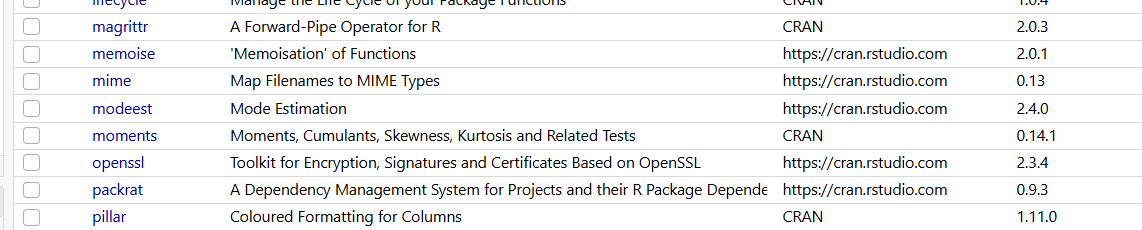
\includegraphics[width=6.77083in,height=\textheight,keepaspectratio]{images/clipboard-2851960019.png}

To install \texttt{mosaic} run the code chunk below. The
\texttt{require} check makes this safe to run multiple times.

\begin{Shaded}
\begin{Highlighting}[]
\ControlFlowTok{if}\NormalTok{ (}\SpecialCharTok{!}\FunctionTok{require}\NormalTok{(}\StringTok{"mosaicData"}\NormalTok{, }\AttributeTok{quietly=}\ConstantTok{TRUE}\NormalTok{)) \{}
  \FunctionTok{install.packages}\NormalTok{(}\StringTok{"mosaicData"}\NormalTok{)}
\NormalTok{\}}
\end{Highlighting}
\end{Shaded}

Now load the \texttt{mosaic} library and import the \texttt{TenMileRace}
data frame.

\begin{Shaded}
\begin{Highlighting}[]
\FunctionTok{library}\NormalTok{(mosaicData)}
\FunctionTok{data}\NormalTok{(TenMileRace)}
\end{Highlighting}
\end{Shaded}

\paragraph{Task 5}\label{task-5}

To practice what we just did for \texttt{mosaic}, write R code to check
if your computer has the library \texttt{dplyr} installed. If not, then
install it. Then load the \texttt{dplyr} library.

We will use \texttt{dplyr} later in the lab.

\subsection{3. Exploring a Data Frame}\label{exploring-a-data-frame}

You can easily view the \texttt{TenMileRace} data frame by clicking the
\textbf{Environment} tab and double-clicking on TenMileRace. You will
see the data frame pop up.

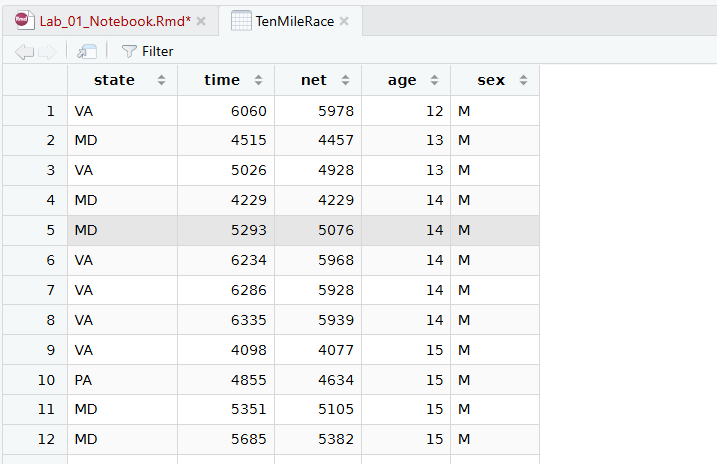
\includegraphics[width=5.47917in,height=\textheight,keepaspectratio]{images/clipboard-4187841108.png}

Try sorting the rows of the data frame by \texttt{time}. Just click on
``time'' once to get ascending order.

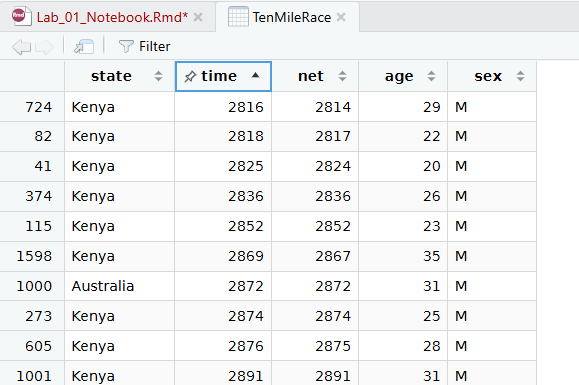
\includegraphics[width=4.41667in,height=\textheight,keepaspectratio]{images/clipboard-1836253605.png}

The variable \texttt{time} is the time taken (in seconds) for an
individual runner to complete the ten-mile Cherry Blossom Race in 2005.


\includegraphics[width=1.76042in,height=\textheight,keepaspectratio]{images/clipboard-2975840456.png}

To find out more about this data set, open the help file by running
\texttt{help(TenMileRace)}.

\begin{Shaded}
\begin{Highlighting}[]
  \FunctionTok{help}\NormalTok{(TenMileRace)}
\end{Highlighting}
\end{Shaded}

The help file explains where the data set comes from and what each
variable (i.e., column) in the data frame represents. Note that
\texttt{net} is described as:

\begin{quote}
The recorded time (in seconds) from when the runner \ul{crossed the
starting line} to when the runner \ul{crossed the finish line}.
\end{quote}

For slower runners who started far back in the crowd, their \texttt{net}
result better represents their race performance than the official
\texttt{time} result.

We can confirm that their were 8636 runners by counting the number of
rows in the data frame with \texttt{nrow}:

\begin{Shaded}
\begin{Highlighting}[]
\FunctionTok{nrow}\NormalTok{(TenMileRace)}
\end{Highlighting}
\end{Shaded}

\begin{verbatim}
## [1] 8636
\end{verbatim}

Based on our quick look at the data, we can see that the race had 8636
runners and it was won by a 29-year old Male from Kenya, who finished
the race in a time of \(2816\) seconds (i.e., \(46\) min \(56\)
seconds).

Now unsort the data frame by clicking the ``time'' header two more times
until you see the rows in their original order:

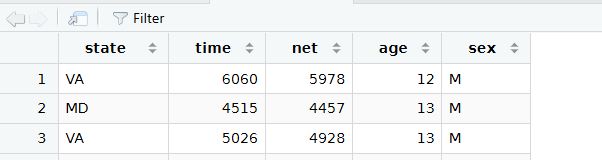
\includegraphics[width=4.21875in,height=\textheight,keepaspectratio]{images/clipboard-1631050950.png}

\subsubsection{Extracting Specific Variable
Values}\label{extracting-specific-variable-values}

Suppose we want to pull out the \texttt{time} for the first runner in
the data frame (who we can see in the previous image is a 12-year old
Male from VA state). One way is to specify the row (1) and column (2) of
that piece of data.

\begin{Shaded}
\begin{Highlighting}[]
\NormalTok{TenMileRace[}\DecValTok{1}\NormalTok{, }\DecValTok{2}\NormalTok{]}
\end{Highlighting}
\end{Shaded}

\begin{verbatim}
## [1] 6060
\end{verbatim}

Another way is to use the \emph{name} of the column:

\begin{Shaded}
\begin{Highlighting}[]
\NormalTok{TenMileRace[}\DecValTok{1}\NormalTok{, }\StringTok{"time"}\NormalTok{]}
\end{Highlighting}
\end{Shaded}

\begin{verbatim}
## [1] 6060
\end{verbatim}

If we wanted to pull out the first five runner times, we could use:

\begin{Shaded}
\begin{Highlighting}[]
\NormalTok{TenMileRace[}\FunctionTok{c}\NormalTok{(}\DecValTok{1}\NormalTok{, }\DecValTok{2}\NormalTok{, }\DecValTok{3}\NormalTok{, }\DecValTok{4}\NormalTok{, }\DecValTok{5}\NormalTok{), }\StringTok{"time"}\NormalTok{]}
\end{Highlighting}
\end{Shaded}

\begin{verbatim}
## [1] 6060 4515 5026 4229 5293
\end{verbatim}

Side note: in R, we can specify a list of numbers using the \texttt{c()}
function, as in

\begin{Shaded}
\begin{Highlighting}[]
\FunctionTok{c}\NormalTok{(}\DecValTok{3}\NormalTok{, }\DecValTok{6}\NormalTok{, }\DecValTok{8}\NormalTok{, }\DecValTok{10}\NormalTok{)}
\end{Highlighting}
\end{Shaded}

\begin{verbatim}
## [1]  3  6  8 10
\end{verbatim}

Or, you can specify a list of consecutive numbers using the colon (:)
notation.

\begin{Shaded}
\begin{Highlighting}[]
\DecValTok{1}\SpecialCharTok{:}\DecValTok{5}
\end{Highlighting}
\end{Shaded}

\begin{verbatim}
## [1] 1 2 3 4 5
\end{verbatim}

\paragraph{Task 6}\label{task-6}

Write an expression to return the \texttt{state} for the first 50
runners in the data frame.

\subsubsection{Extracting Entire
Variable}\label{extracting-entire-variable}

If you want to get the entire variable \texttt{time}, you can use the \$
syntax. This would give a very long output, so we will store the
\texttt{time} values into a new variable called \texttt{race.times}.

\begin{Shaded}
\begin{Highlighting}[]
\NormalTok{race.times }\OtherTok{\textless{}{-}}\NormalTok{ TenMileRace}\SpecialCharTok{$}\NormalTok{time}
\end{Highlighting}
\end{Shaded}

\textbf{R Note:} Variable assignment uses the ``arrow'' symbol
\texttt{\textless{}-} in R. Also, R does \emph{not} use the dot operator
(\texttt{.}) the same way as C or Java or python. In R, the dot is often
used in variable names.

This gives a new way to pull out the first five race times:

\begin{Shaded}
\begin{Highlighting}[]
\NormalTok{race.times[}\DecValTok{1}\SpecialCharTok{:}\DecValTok{5}\NormalTok{]}
\end{Highlighting}
\end{Shaded}

\begin{verbatim}
## [1] 6060 4515 5026 4229 5293
\end{verbatim}

\subsubsection{Frequency Table}\label{frequency-table}

For non-numerical variables like \texttt{sex}, the possible values of
the variable (``M'' and ``F'') are called \emph{levels} in R.

\begin{Shaded}
\begin{Highlighting}[]
\FunctionTok{levels}\NormalTok{(TenMileRace}\SpecialCharTok{$}\NormalTok{sex)}
\end{Highlighting}
\end{Shaded}

\begin{verbatim}
## [1] "F" "M"
\end{verbatim}

The best way to summarize a non-numerical variable like \texttt{sex} is
with a \emph{frequency table}, which simply counts how many times each
level occurs for that variable in the data set.

\begin{Shaded}
\begin{Highlighting}[]
\FunctionTok{table}\NormalTok{( TenMileRace}\SpecialCharTok{$}\NormalTok{sex )}
\end{Highlighting}
\end{Shaded}

\begin{verbatim}
## 
##    F    M 
## 4325 4311
\end{verbatim}

This shows that there were \(4325\) female runners and \(4311\) male
runners in the race.

\subsubsection{Logical Arrays}\label{logical-arrays}

It is often useful to check if a numerical variable satisfies a certain
condition. This can generate an array of \emph{Boolean} (i.e., logical)
values.

\begin{Shaded}
\begin{Highlighting}[]
\NormalTok{  TenMileRace}\SpecialCharTok{$}\NormalTok{time }\SpecialCharTok{\textless{}} \DecValTok{3000}
\end{Highlighting}
\end{Shaded}

That generated a very long Boolean array. To see just the first few
values use \texttt{head}.

\begin{Shaded}
\begin{Highlighting}[]
\FunctionTok{head}\NormalTok{(TenMileRace}\SpecialCharTok{$}\NormalTok{time }\SpecialCharTok{\textless{}} \DecValTok{3000}\NormalTok{)}
\end{Highlighting}
\end{Shaded}

\begin{verbatim}
## [1] FALSE FALSE FALSE FALSE FALSE FALSE
\end{verbatim}

This shows that none of the first six runners had a time below 3000
seconds.

A Boolean array can be used to specify which rows to pull out of the
data frame. The following returns the \texttt{time} values of all
runners below 3000 seconds.

\begin{Shaded}
\begin{Highlighting}[]
\NormalTok{TenMileRace[TenMileRace}\SpecialCharTok{$}\NormalTok{time }\SpecialCharTok{\textless{}} \DecValTok{3000}\NormalTok{, }\StringTok{"time"}\NormalTok{ ]}
\end{Highlighting}
\end{Shaded}

\begin{verbatim}
##  [1] 2825 2818 2852 2933 2874 2836 2961 2999 2899 2963 2876 2816 2872 2891 2869
\end{verbatim}

Here is another way to get the same \texttt{time} values:

\begin{Shaded}
\begin{Highlighting}[]
\NormalTok{TenMileRace}\SpecialCharTok{$}\NormalTok{time[ TenMileRace}\SpecialCharTok{$}\NormalTok{time }\SpecialCharTok{\textless{}} \DecValTok{3000}\NormalTok{ ]}
\end{Highlighting}
\end{Shaded}

\begin{verbatim}
##  [1] 2825 2818 2852 2933 2874 2836 2961 2999 2899 2963 2876 2816 2872 2891 2869
\end{verbatim}

To get the entire \emph{row} of variables (not just the \texttt{time})
for those runners, we can omit the ``time'' in the second index
position, and R will return a new data frame containing the entire rows
for those runners. We will call this the ``fast runners'' subset.

\begin{Shaded}
\begin{Highlighting}[]
\NormalTok{fast.runners }\OtherTok{\textless{}{-}}\NormalTok{ TenMileRace[TenMileRace}\SpecialCharTok{$}\NormalTok{time }\SpecialCharTok{\textless{}} \DecValTok{3000}\NormalTok{,  ]}
\NormalTok{fast.runners}
\end{Highlighting}
\end{Shaded}

\begin{verbatim}
##          state time  net age sex
## 41       Kenya 2825 2824  20   M
## 82       Kenya 2818 2817  22   M
## 115      Kenya 2852 2852  23   M
## 116   Ethiopia 2933 2933  23   M
## 273      Kenya 2874 2874  25   M
## 374      Kenya 2836 2836  26   M
## 375  Lithuania 2961 2961  26   M
## 376   Colombia 2999 2998  26   M
## 484      Japan 2899 2899  27   M
## 485      Kenya 2963 2962  27   M
## 605      Kenya 2876 2875  28   M
## 724      Kenya 2816 2814  29   M
## 1000 Australia 2872 2872  31   M
## 1001     Kenya 2891 2891  31   M
## 1598     Kenya 2869 2867  35   M
\end{verbatim}

How many fast runners are there? Recall that we can count the number of
rows using \texttt{nrow}:

\begin{Shaded}
\begin{Highlighting}[]
\FunctionTok{nrow}\NormalTok{(fast.runners)}
\end{Highlighting}
\end{Shaded}

\begin{verbatim}
## [1] 15
\end{verbatim}

A direct way to count how many fast runners there are (with
\texttt{time\ \textless{}\ 3000}) uses \texttt{sum}. This way works
because False = 0 and True = 1.

\begin{Shaded}
\begin{Highlighting}[]
\FunctionTok{sum}\NormalTok{( TenMileRace}\SpecialCharTok{$}\NormalTok{time }\SpecialCharTok{\textless{}} \DecValTok{3000}\NormalTok{)}
\end{Highlighting}
\end{Shaded}

\begin{verbatim}
## [1] 15
\end{verbatim}

\paragraph{Task 7}\label{task-7}

Write an expression that returns a data frame for all runner from the
\texttt{state} of ``Ethiopia''.

\paragraph{Task 8}\label{task-8}

Write an R expression to return the \texttt{sex} of all ``slow
runners'', meaning those with \texttt{net} time \emph{larger} than
10,000 seconds. How many such runners are there?

\subsubsection{Subsetting}\label{subsetting}

Pulling rows out of data frame based on certain conditions is needed
frequently. We can conveniently perform the same task using the
\texttt{subset} function.

\begin{Shaded}
\begin{Highlighting}[]
\NormalTok{slow.runners }\OtherTok{\textless{}{-}} \FunctionTok{subset}\NormalTok{( TenMileRace, net }\SpecialCharTok{\textgreater{}} \DecValTok{10000}\NormalTok{ )}
\end{Highlighting}
\end{Shaded}

If there are multiple conditions, you can combine them using logical
operations

\begin{itemize}
\item
  AND (\texttt{\&)}
\item
  OR (\texttt{\textbar{}})
\item
  NOT (\texttt{!})
\end{itemize}

For example, here is the data frame for all Female runners older than 65
who were not from Virginia (VA).

\begin{Shaded}
\begin{Highlighting}[]
\FunctionTok{subset}\NormalTok{(TenMileRace, (sex}\SpecialCharTok{==}\StringTok{"F"}\NormalTok{) }\SpecialCharTok{\&}\NormalTok{ (age}\SpecialCharTok{\textgreater{}}\DecValTok{65}\NormalTok{) }\SpecialCharTok{\&} \SpecialCharTok{!}\NormalTok{(state}\SpecialCharTok{==}\StringTok{"VA"}\NormalTok{))}
\end{Highlighting}
\end{Shaded}

\begin{verbatim}
##      state time  net age sex
## 8628    MA 5212 5103  66   F
## 8629    MD 6453 6363  66   F
## 8630    NJ 5111 5099  68   F
## 8631    MD 5715 5705  68   F
## 8633    NY 5680 5667  72   F
## 8634    DC 7401 7401  73   F
## 8635    ND 9726 9231  75   F
\end{verbatim}

\paragraph{Task 9}\label{task-9}

Use \texttt{subset} to write an R expression that returns all rows of
\texttt{TenMileRace} with runners whose \texttt{net} is between 3000
seconds and 10000 seconds (including endpoints). Assign this to a
variable \texttt{mid.runners}. Then write an expression to return the
number of runners in this subset.

\paragraph{Task 10}\label{task-10}

Use \texttt{subset} to pull out the data frame containing all Female
(``F'') runners from Russia or Kenya.

\paragraph{Task 11}\label{task-11}

Write R code to obtain the data frame of all runners who are \emph{not}
from the USA. How many such runners are there?

\emph{Hint: the state codes for all USA runners are exactly two
characters (like ``VA''). Use \texttt{nchar(as.character(state))} to
count the number of characters.}

\subsubsection{\texorpdfstring{Using
\texttt{droplevels}}{Using droplevels}}\label{using-droplevels}

Suppose we want to select all the runners from the states of ``VA'',
``MD'', and ``DC''. We can do this using logical OR or using the
\texttt{\%in\%} operator.

\begin{Shaded}
\begin{Highlighting}[]
\CommentTok{\#subset( TenMileRace, (state == "VA") | (state == "MD") | (state == "DC"))}
\end{Highlighting}
\end{Shaded}

\begin{Shaded}
\begin{Highlighting}[]
\NormalTok{my.subset }\OtherTok{\textless{}{-}} \FunctionTok{subset}\NormalTok{( TenMileRace, state }\SpecialCharTok{\%in\%} \FunctionTok{c}\NormalTok{(}\StringTok{"VA"}\NormalTok{, }\StringTok{"MD"}\NormalTok{, }\StringTok{"DC"}\NormalTok{))}
\end{Highlighting}
\end{Shaded}

Now suppose we make a frequency table for the \texttt{state} of
\texttt{my.subset}. Strangely, the table contains \emph{all} the
original levels of \texttt{state} but with counts of 0.

\begin{Shaded}
\begin{Highlighting}[]
\FunctionTok{table}\NormalTok{(my.subset}\SpecialCharTok{$}\NormalTok{state)}
\end{Highlighting}
\end{Shaded}

\begin{verbatim}
## 
##                      AK          AL          AR   Australia          AZ 
##           0           0           0           0           0           0 
##          CA          CO    Colombia          CT          DC          DE 
##           0           0           0           0        1642           0 
##          EN    Ethiopia          FL          GA          GE          HI 
##           0           0           0           0           0           0 
##          IA          IL          IM          IN       Japan       Kenya 
##           0           0           0           0           0           0 
##          KS          KY          LA          LE   Lithuania          MA 
##           0           0           0           0           0           0 
##          MD          ME          MI          MN          MO          NC 
##        2166           0           0           0           0           0 
##          ND          NE New Zealand          NH          NJ          NM 
##           0           0           0           0           0           0 
##          NY          OH          OR          PA          RI     Romania 
##           0           0           0           0           0           0 
##      Russia          SA          SC          TN          TX    Uhwiesen 
##           0           0           0           0           0           0 
##     Ukraine         Usa          VA          VI          VT          WA 
##           0           0        3689           0           0           0 
##          WI          WV 
##           0           0
\end{verbatim}

To force R to forget the old levels of \texttt{state} that are now
empty, use the function \texttt{droplevels}.

\begin{Shaded}
\begin{Highlighting}[]
\NormalTok{my.subset }\OtherTok{\textless{}{-}} \FunctionTok{droplevels}\NormalTok{( my.subset )}
\FunctionTok{table}\NormalTok{(my.subset}\SpecialCharTok{$}\NormalTok{state)}
\end{Highlighting}
\end{Shaded}

\begin{verbatim}
## 
##   DC   MD   VA 
## 1642 2166 3689
\end{verbatim}

\paragraph{Task 12}\label{task-12}

Use \texttt{subset} and \texttt{droplevels} and \texttt{table} to
produce a frequency table showing the number of USA runners from each
state. (The table should not show any other \texttt{state} categories.)

\paragraph{Task 13}\label{task-13}

\textbf{Challenging} Use the function \texttt{which.max} (and other
stuff) to print out which US state had the most runners. \emph{Hint:
help(which.max)}

\subsection{\texorpdfstring{Filtering with
\texttt{dplyr}}{Filtering with dplyr}}\label{filtering-with-dplyr}

The library \texttt{dplyr} provides a useful function, \texttt{filter},
which is an alternative to the \texttt{subset} function. Make sure you
have loaded the \texttt{dplyr} library.

\begin{Shaded}
\begin{Highlighting}[]
\FunctionTok{library}\NormalTok{(dplyr)}
\end{Highlighting}
\end{Shaded}

\begin{verbatim}
## 
## Attaching package: 'dplyr'
\end{verbatim}

\begin{verbatim}
## The following objects are masked from 'package:stats':
## 
##     filter, lag
\end{verbatim}

\begin{verbatim}
## The following objects are masked from 'package:base':
## 
##     intersect, setdiff, setequal, union
\end{verbatim}

The function \texttt{filter} works like \texttt{subset} except you
simply list the various conditions as separate arguments (no logical AND
needed). For example, to get rows for Female runners from VA with net
time below 4000 seconds, use

\begin{Shaded}
\begin{Highlighting}[]
\FunctionTok{filter}\NormalTok{(TenMileRace, sex }\SpecialCharTok{==} \StringTok{"F"}\NormalTok{, state }\SpecialCharTok{==} \StringTok{"VA"}\NormalTok{, net }\SpecialCharTok{\textless{}} \DecValTok{4000}\NormalTok{)}
\end{Highlighting}
\end{Shaded}

\begin{verbatim}
##    state time  net age sex
## 1     VA 3460 3457  23   F
## 2     VA 3843 3827  23   F
## 3     VA 4018 3995  23   F
## 4     VA 3837 3837  25   F
## 5     VA 3660 3657  29   F
## 6     VA 3723 3723  29   F
## 7     VA 4003 3983  30   F
## 8     VA 3784 3781  32   F
## 9     VA 3447 3447  33   F
## 10    VA 3804 3803  33   F
## 11    VA 3867 3854  40   F
## 12    VA 3896 3896  43   F
## 13    VA 3884 3881  44   F
\end{verbatim}

\paragraph{Task 14}\label{task-14}

Use \texttt{filter} to get a data frame containing all Male runners who
are \emph{not} from ``VA'' and \emph{not} from ``MD''.

\subsection{4. Sample Statistics}\label{sample-statistics}

For numerical variables like \texttt{net}, we typically calculate
\emph{sample statistics} to get a clearer understanding of the variable.

For example, to understand what a typical \texttt{net} time is for the
Cherry Blossom Race, we calculate the \emph{mean} and \emph{median}.

\begin{Shaded}
\begin{Highlighting}[]
\NormalTok{race.times }\OtherTok{\textless{}{-}}\NormalTok{ TenMileRace}\SpecialCharTok{$}\NormalTok{net }
\FunctionTok{mean}\NormalTok{( race.times )}
\end{Highlighting}
\end{Shaded}

\begin{verbatim}
## [1] 5599.065
\end{verbatim}

\begin{Shaded}
\begin{Highlighting}[]
\FunctionTok{median}\NormalTok{( race.times)}
\end{Highlighting}
\end{Shaded}

\begin{verbatim}
## [1] 5555
\end{verbatim}

Note that these numbers are about 44 seconds different from each other.
Either way, a typical \texttt{net} time is about 93 minutes (which is
5580 seconds).

We can also calculate the minimum and maximum race times use
\texttt{min} and \texttt{max}.

\begin{Shaded}
\begin{Highlighting}[]
\FunctionTok{min}\NormalTok{( race.times ) }
\end{Highlighting}
\end{Shaded}

\begin{verbatim}
## [1] 2814
\end{verbatim}

\begin{Shaded}
\begin{Highlighting}[]
\FunctionTok{max}\NormalTok{( race.times )}
\end{Highlighting}
\end{Shaded}

\begin{verbatim}
## [1] 10536
\end{verbatim}

\paragraph{Task 15}\label{task-15}

Use \texttt{filter} and \texttt{mean} to calculate separately the
average Male and Female \texttt{net} times.

\paragraph{Task 16}\label{task-16}

Calculate the mean \texttt{net} time of all local runners (meaning
runners from the state ``MD'', ``VA'', or ``DC'') and all non-local
runners.

On average, were local runners faster or slower than all other runners?

\paragraph{Task 17}\label{task-17}

Write R code to count the number of Male runners who finished before the
fastest Female runner (based on \texttt{time}, not \texttt{net}). Do not
hard-code any literal numbers in your code!

\subsection{Rank Statistic}\label{rank-statistic}

The \emph{rank} of an individual runner's \texttt{net} time is their
\emph{numerical position} (1st, 2nd, 3rd, \ldots) of finishing the race.
If I finished first, then my rank is 1. In the case of a tie, more than
one runner can get the same rank.

In this example, the first and third values are tied for 1st and the
second and fifth values are tied for 3rd.

\begin{Shaded}
\begin{Highlighting}[]
\FunctionTok{rank}\NormalTok{( }\FunctionTok{c}\NormalTok{(}\DecValTok{50}\NormalTok{, }\DecValTok{200}\NormalTok{, }\DecValTok{50}\NormalTok{, }\DecValTok{400}\NormalTok{, }\DecValTok{200}\NormalTok{, }\DecValTok{700}\NormalTok{), }\AttributeTok{ties.method=}\StringTok{"min"}\NormalTok{)}
\end{Highlighting}
\end{Shaded}

\begin{verbatim}
## [1] 1 3 1 5 3 6
\end{verbatim}

In the Cherry Blossom Race, the first few runners in the data frame have
ranks as shown.

\begin{Shaded}
\begin{Highlighting}[]
\FunctionTok{head}\NormalTok{(}\FunctionTok{rank}\NormalTok{( TenMileRace}\SpecialCharTok{$}\NormalTok{net, }\AttributeTok{ties.method=}\StringTok{"min"}\NormalTok{ ))}
\end{Highlighting}
\end{Shaded}

\begin{verbatim}
## [1] 5897  944 2111  577 2526 5854
\end{verbatim}

\paragraph{Task 18}\label{task-18}

Write R code to get the data frame containing the top 100 runners by
rank (using \texttt{time}. Then calculate the mean \texttt{time} and the
mean \texttt{net} for those runners.

\paragraph{Task 19}\label{task-19}

Every runner's \texttt{net} time is either equal to or less than their
\texttt{time} (gun time). Find the top 5 runners whose \texttt{net} time
is the furthest below their \texttt{time}. Print those runner's
\texttt{state}, \texttt{age}, and \texttt{sex}.

\subsubsection{Histograms}\label{histograms}

The most important type of graph or chart to present a numerical
variable \(X\) is the \emph{histogram}. It shows how many individuals
had an \(X\) value falling within a sequence of pre-determined ``bins''
or ``classes''.

For instance, all the \texttt{net} times in \texttt{TenMileRace} fall
between 2800 and 10600. We can divide this into 78 classes as follows:

{[}2800, 2900),

{[}2900, 3000),

{[}3000, 3100),

\ldots{}

{[}10400, 10500),

{[}10500, 10600)

The round brackets indicate that the right endpoint is \emph{not}
included in that class. We can then determine the frequency (i.e.,
count) of how many runners' \texttt{net} time falls into each class and
then plot a vertical rectangle showing the frequency for each class. The
result is a histogram of \texttt{net} times.

\begin{Shaded}
\begin{Highlighting}[]
\FunctionTok{hist}\NormalTok{( TenMileRace}\SpecialCharTok{$}\NormalTok{net, }\AttributeTok{breaks=}\FunctionTok{seq}\NormalTok{(}\DecValTok{2800}\NormalTok{, }\DecValTok{10600}\NormalTok{, }\AttributeTok{by=}\DecValTok{100}\NormalTok{), }\AttributeTok{right =} \ConstantTok{FALSE}\NormalTok{,}
      \AttributeTok{xlab=}\StringTok{"net (seconds)"}\NormalTok{, }
      \AttributeTok{main=}\StringTok{"net times in Cherry Blossom Race (n = 8636)"}\NormalTok{)}
\end{Highlighting}
\end{Shaded}

\pandocbounded{\includegraphics[keepaspectratio]{Lab_01_Notebook_files/figure-latex/unnamed-chunk-51-1.pdf}}

Using a class width of 200 instead of 100 creates a smoother shape with
wider rectangles:

\begin{Shaded}
\begin{Highlighting}[]
\FunctionTok{hist}\NormalTok{( TenMileRace}\SpecialCharTok{$}\NormalTok{net, }\AttributeTok{breaks=}\FunctionTok{seq}\NormalTok{(}\DecValTok{2800}\NormalTok{, }\DecValTok{10600}\NormalTok{, }\AttributeTok{by=}\DecValTok{200}\NormalTok{), }\AttributeTok{right =} \ConstantTok{FALSE}\NormalTok{,}
      \AttributeTok{xlab=}\StringTok{"net (seconds)"}\NormalTok{, }
      \AttributeTok{main=}\StringTok{"net times in Cherry Blossom Race (n = 8636)"}\NormalTok{)}
\end{Highlighting}
\end{Shaded}

\pandocbounded{\includegraphics[keepaspectratio]{Lab_01_Notebook_files/figure-latex/unnamed-chunk-52-1.pdf}}

\paragraph{Task 20}\label{task-20}

Define the \emph{usual} runners to be those runners who were \emph{not}
the slowest 5\% and \emph{not} the fastest 5\% of runners (based on
\texttt{net} time).

Use \texttt{filter} and \texttt{rank} to extract all the usual runners.
Then generate a histogram with a class width of 300 seconds (i.e., 5
minutes) to present all the usual runners. Find out how to make the
rectangles pink.

\section{Pencil Problems}\label{pencil-problems}

These problems are meant to be done with paper and pencil (and
scientific calculator). They will help you prepare for the theory part
of the quiz and the exams.

\begin{enumerate}
\def\labelenumi{\arabic{enumi}.}
\item
  To test new equipment for making ¾'' plywood, 18 measurements of
  thickness \(X\) were obtained. Calculate the mean, median, range, and
  standard deviation of \(X\) based on the sample data. Measurements
  below are in inches.

  {\def\LTcaptype{none} % do not increment counter
  \begin{longtable}[]{@{}
    >{\raggedright\arraybackslash}p{(\linewidth - 16\tabcolsep) * \real{0.1111}}
    >{\raggedright\arraybackslash}p{(\linewidth - 16\tabcolsep) * \real{0.1111}}
    >{\raggedright\arraybackslash}p{(\linewidth - 16\tabcolsep) * \real{0.1111}}
    >{\raggedright\arraybackslash}p{(\linewidth - 16\tabcolsep) * \real{0.1111}}
    >{\raggedright\arraybackslash}p{(\linewidth - 16\tabcolsep) * \real{0.1111}}
    >{\raggedright\arraybackslash}p{(\linewidth - 16\tabcolsep) * \real{0.1111}}
    >{\raggedright\arraybackslash}p{(\linewidth - 16\tabcolsep) * \real{0.1111}}
    >{\raggedright\arraybackslash}p{(\linewidth - 16\tabcolsep) * \real{0.1111}}
    >{\raggedright\arraybackslash}p{(\linewidth - 16\tabcolsep) * \real{0.1111}}@{}}
  \toprule\noalign{}
  \endhead
  \bottomrule\noalign{}
  \endlastfoot
  0.754 & 0.735 & 0.754 & 0.748 & 0.740 & 0.752 & 0.747 & 0.740 &
  0.751 \\
  0.741 & 0.740 & 0.742 & 0.748 & 0.732 & 0.750 & 0.747 & 0.750 &
  0.752 \\
  \end{longtable}
  }
\item
  Calculate the mean and standard deviation of the diameter \(X\) of
  steel rods from a sample of 350 rods.

  {\def\LTcaptype{none} % do not increment counter
  \begin{longtable}[]{@{}ll@{}}
  \toprule\noalign{}
  \textbf{Diameter (mm)} & \textbf{Frequency} \\
  \midrule\noalign{}
  \endhead
  \bottomrule\noalign{}
  \endlastfoot
  10.00 & 40 \\
  10.01 & 75 \\
  10.02 & 100 \\
  10.03 & 90 \\
  10.04 & 45 \\
  \end{longtable}
  }
\item
  The daily opening price of gold (C\$ per oz) for the last ten days of
  Aug 2026 are given below.

  \begin{enumerate}
  \def\labelenumii{\alph{enumii}.}
  \item
    Determine the typical price of gold over this time period. Provide
    more than one measure.
  \item
    Calculate the standard deviation of gold Price based on the data
    given. What is the typical amount that the Price of gold deviates on
    any given day from its background value? (This is one measure of
    \emph{volitility}.)
  \item
    If gold Price is a normally distributed variable, then it is very
    unlikely to go outside three standard deviations above or below the
    mean Price. What are these upper and lower Prices, and what is the
    probability that the gold Price goes outside these limits just by
    chance?

    {\def\LTcaptype{none} % do not increment counter
    \begin{longtable}[]{@{}l@{}}
    \toprule\noalign{}
    \textbf{Price of Gold (CA\$ per oz)} \\
    \midrule\noalign{}
    \endhead
    \bottomrule\noalign{}
    \endlastfoot
    6195.20 \\
    6377.58 \\
    6374.78 \\
    6448.51 \\
    6439.12 \\
    6343.34 \\
    6231.64 \\
    6244.87 \\
    6023.88 \\
    6127.91 \\
    \end{longtable}
    }
  \end{enumerate}
\item
  Hank and Pete work in a fabrication facility. Records indicate that
  Hank completes an average of 62 items per shift, with a standard
  deviation of 4.2 items. Pete completes an average of 59 items per
  shift, with a standard deviation of 4.1 items. Which of the two would
  you consider to be the more consistent worker? Explain.
\item
  Suppose a lumber mill ships 4x4's with a mean moisture content of
  \(\mu=18\%\) and \(\sigma=0.5\%\). A histogram reveals that the data
  is bell-shaped.

  \begin{enumerate}
  \def\labelenumii{\alph{enumii}.}
  \item
    Use Chebyshev's Rule to determine the minimum percentage of scores
    that lie between 17\% and 19\%.
  \item
    Repeat question a. using the ``Empirical Rule''.
  \item
    Use the Empirical Rule to estimate the percentage of values greater
    than 19.5\%.
  \item
    Use the Empirical Rule to estimate the percentage of values between
    18\% and 18.5\%.
  \item
    Building specifications require that the moisture content be under
    19\% to be closed in. Use the Empirical Rule to estimate the
    percentage of 4x4's that are suitable to be closed in.
  \end{enumerate}
\item
  Human body temperatures have a mean of \(98.20 ^\circ F\) and a
  standard deviation of \(0.62 ^\circ F\). Determine whether each of the
  following temperatures is usual or unusual:

  {\def\LTcaptype{none} % do not increment counter
  \begin{longtable}[]{@{}lll@{}}
  \toprule\noalign{}
  \endhead
  \bottomrule\noalign{}
  \endlastfoot
  \(101.00 ^\circ F\) & \(96.90 ^\circ F\) & \(96.98 ^\circ F\) \\
  \end{longtable}
  }
\item
  The two sets of sample data below (Site A and Site B) are measurements
  of the drainage rate of the soil in two different building sites (in
  \(litre / m^2\cdot s\)).

  \begin{enumerate}
  \def\labelenumii{\alph{enumii}.}
  \tightlist
  \item
    Based on relevant sample statistics, which of the sites has better
    drainage (higher and more consistent)? Conclude which site you would
    be more likely to recommend constructing a building on.
  \item
    For Site B data set, assume that the drainage rates are known to be
    distributed in a bell-shaped curve. Could either (or both) the max
    and min values could be discounted as being too extreme?
  \item
    If you were to exclude the minimum data point from the data set for
    site A, what would be the effect on the mean and the standard
    deviation?
  \end{enumerate}

  {\def\LTcaptype{none} % do not increment counter
  \begin{longtable}[]{@{}ll@{}}
  \toprule\noalign{}
  \emph{Site A} & \emph{Site B} \\
  \midrule\noalign{}
  \endhead
  \bottomrule\noalign{}
  \endlastfoot
  2.99 & 1.02 \\
  4.75 & 3.56 \\
  8.79 & 3.5 \\
  5.59 & 3.45 \\
  2.32 & 4.5 \\
  1.9 & 13.6 \\
  & 4.5 \\
  & 2.3 \\
  & 3.5 \\
  & 2.6 \\
  & 3.31 \\
  & 3.1 \\
  \end{longtable}
  }
\end{enumerate}

\end{document}
